\documentclass[../../main.tex]{subfiles}
\begin{document}
\section{Validity of a model for a cantilever two-dimensional beam} \label{sec:validity-of-a-2d-beam}

In Section \ref{sec:validity-of-a-cantilever-timoshenko-beam}, the article \cite{LVV09} was discussed. In this article, the authors investigated the validity of a cantilever Timoshenko beam by comparing it to a cantilever two-dimensional beam. In this section, the article is extended and the validity of the cantilever two-dimensional model is investigated.

As mentioned in the introduction of the chapter, a beam is a three-dimensional body and therefore a three-dimensional model is more realistic. However the authors of \cite{LVV09} mention that a direct comparison of the one and three-dimensional models will have complexities and they suggest using the two-dimensional model as an intermediate step.

So in this section, the article \cite{LVV09} is extended and the validity of a cantilever two-dimensional beam model is investigated, using a cantilever three-dimensional model as a reference.

\subsection{The models}
The two-dimensional model is the same model as used in the previous section, Problem T-2 defined in Section \ref{ssec:2D_Model:ModelProblem}. From Section \ref{ssec:3D_Model:ModelProblems}, the cantilever three-dimensional model, referred to as Problem 3D-1.

Figure \ref{fig:2Dv3D} shows the two beams side-by-side.

\FloatBarrier
\begin{figure}[h!]
	\scalebox{.8}{
		\makebox[\textwidth][c]{
			\caption{Side-by-side comparison of the beams.}
			\label{fig:2Dv3D}
			\centering
			\begin{minipage}[b]{0.7\linewidth}
				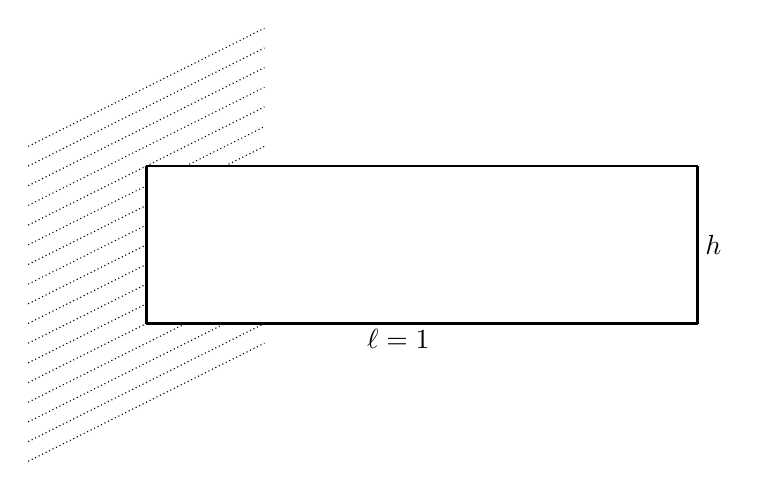
\begin{tikzpicture}
					\draw[line width = 0.3mm] (0,1) -- (7,1);
					\draw[line width = 0.3mm] (0,-1) -- (7,-1);
					\draw[line width = 0.3mm] (7,-1) -- (7,1);
					\draw[line width = 0.3mm] (0,-1) -- (0,1);
					
					
					\draw[scale=0.5, domain=-3:3, smooth, variable=\x,densely dotted] plot ({\x}, {0.5*\x+4});
					\draw[scale=0.5, domain=-3:3, smooth, variable=\x,densely dotted] plot ({\x}, {0.5*\x+3.5});
					\draw[scale=0.5, domain=-3:3, smooth, variable=\x,densely dotted] plot ({\x}, {0.5*\x+3});
					\draw[scale=0.5, domain=-3:3, smooth, variable=\x,densely dotted] plot ({\x}, {0.5*\x+2.5});
					\draw[scale=0.5, domain=-3:3, smooth, variable=\x,densely dotted] plot ({\x}, {0.5*\x+2});
					
					\draw[scale=0.5, domain=-3:0, smooth, variable=\x,densely dotted] plot ({\x}, {0.5*\x+1.5});
					\draw[scale=0.5, domain=-3:0, smooth, variable=\x,densely dotted] plot ({\x}, {0.5*\x+1});
					
					
					\draw[scale=0.5, domain=1:3, smooth, variable=\x,densely dotted] plot ({\x}, {0.5*\x+1.5});
					\draw[scale=0.5, domain=2:3, smooth, variable=\x,densely dotted] plot ({\x}, {0.5*\x+1});
					
					\draw[scale=0.5, domain=-3:0, smooth, variable=\x,densely dotted] plot ({\x}, {0.5*\x+0.5});
					\draw[scale=0.5, domain=-3:0, smooth, variable=\x,densely dotted] plot ({\x}, {0.5*\x});
					\draw[scale=0.5, domain=-3:0, smooth, variable=\x,densely dotted] plot ({\x}, {0.5*\x-0.5});
					\draw[scale=0.5, domain=-3:0, smooth, variable=\x,densely dotted] plot ({\x}, {0.5*\x-1});
					\draw[scale=0.5, domain=-3:0, smooth, variable=\x,densely dotted] plot ({\x}, {0.5*\x-1.5});
					\draw[scale=0.5, domain=-3:0, smooth, variable=\x,densely dotted] plot ({\x}, {0.5*\x-2});
					\draw[scale=0.5, domain=-3:1, smooth, variable=\x,densely dotted] plot ({\x}, {0.5*\x-2.5});
					\draw[scale=0.5, domain=-3:2, smooth, variable=\x,densely dotted] plot ({\x}, {0.5*\x-3});
					\draw[scale=0.5, domain=-3:3, smooth, variable=\x,densely dotted] plot ({\x}, {0.5*\x-3.5});
					\draw[scale=0.5, domain=-3:3, smooth, variable=\x,densely dotted] plot ({\x}, {0.5*\x-4});
					
					\node at (7.2,0) {$h$};
					\node at (3.2,-1.2) {$\ell = 1$};
				\end{tikzpicture}
				\subcaption{Two-Dimensional Elastic Body}
			\end{minipage}
			\begin{minipage}[b]{0.7\linewidth}
				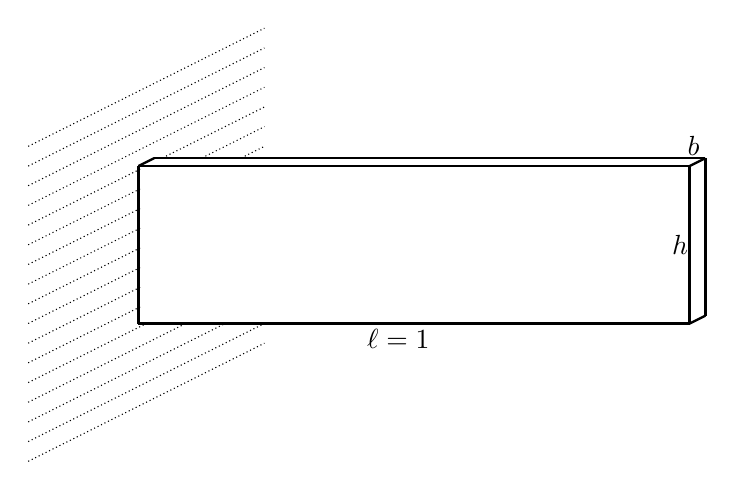
\begin{tikzpicture}
					\draw[line width = 0.3mm] (-0.1,1) -- (6.9,1);
					\draw[line width = 0.3mm] (-0.1,-1) -- (6.9,-1);
					\draw[line width = 0.3mm] (6.9,-1) -- (6.9,1);
					\draw[line width = 0.3mm] (-0.1,-1) -- (-0.1,1);
					
					\draw[line width = 0.3mm] (0.1,1.1) -- (7.1,1.1);
					\draw[line width = 0.3mm] (7.1,-0.9) -- (7.1,1.1);
					
					\draw[line width = 0.3mm] (-0.1,1) -- (0.1,1.1);
					\draw[line width = 0.3mm] (6.9,1) -- (7.1,1.1);
					\draw[line width = 0.3mm] (6.9,-1) -- (7.1,-0.9);
					
					
					
					\draw[scale=0.5, domain=-3:3, smooth, variable=\x,densely dotted] plot ({\x}, {0.5*\x+4});
					\draw[scale=0.5, domain=-3:3, smooth, variable=\x,densely dotted] plot ({\x}, {0.5*\x+3.5});
					\draw[scale=0.5, domain=-3:3, smooth, variable=\x,densely dotted] plot ({\x}, {0.5*\x+3});
					\draw[scale=0.5, domain=-3:3, smooth, variable=\x,densely dotted] plot ({\x}, {0.5*\x+2.5});
					
					\draw[scale=0.5, domain=-3:-0.1, smooth, variable=\x,densely dotted] plot ({\x}, {0.5*\x+2});
					\draw[scale=0.5, domain=-3:-0.1, smooth, variable=\x,densely dotted] plot ({\x}, {0.5*\x+1.5});
					\draw[scale=0.5, domain=-3:-0.1, smooth, variable=\x,densely dotted] plot ({\x}, {0.5*\x+1});
					
					\draw[scale=0.5, domain=0.5:3, smooth, variable=\x,densely dotted] plot ({\x}, {0.5*\x+2});
					\draw[scale=0.5, domain=1.5:3, smooth, variable=\x,densely dotted] plot ({\x}, {0.5*\x+1.5});
					\draw[scale=0.5, domain=2.5:3, smooth, variable=\x,densely dotted] plot ({\x}, {0.5*\x+1});
					
					\draw[scale=0.5, domain=-3:-0.1, smooth, variable=\x,densely dotted] plot ({\x}, {0.5*\x+0.5});
					\draw[scale=0.5, domain=-3:-0.1, smooth, variable=\x,densely dotted] plot ({\x}, {0.5*\x});
					\draw[scale=0.5, domain=-3:-0.1, smooth, variable=\x,densely dotted] plot ({\x}, {0.5*\x-0.5});
					\draw[scale=0.5, domain=-3:-0.1, smooth, variable=\x,densely dotted] plot ({\x}, {0.5*\x-1});
					\draw[scale=0.5, domain=-3:-0.1, smooth, variable=\x,densely dotted] plot ({\x}, {0.5*\x-1.5});
					\draw[scale=0.5, domain=-3:0, smooth, variable=\x,densely dotted] plot ({\x}, {0.5*\x-2});
					\draw[scale=0.5, domain=-3:1, smooth, variable=\x,densely dotted] plot ({\x}, {0.5*\x-2.5});
					\draw[scale=0.5, domain=-3:2, smooth, variable=\x,densely dotted] plot ({\x}, {0.5*\x-3});
					\draw[scale=0.5, domain=-3:3, smooth, variable=\x,densely dotted] plot ({\x}, {0.5*\x-3.5});
					\draw[scale=0.5, domain=-3:3, smooth, variable=\x,densely dotted] plot ({\x}, {0.5*\x-4});
					
					\node at (6.95,1.25) {$b$};
					\node at (6.78,0) {$h$};
					\node at (3.2,-1.2) {$\ell = 1$};
					

				\end{tikzpicture}
				\subcaption{Three-Dimensional Elastic Body}
				
			\end{minipage}
		}
	}
\end{figure}
\FloatBarrier

\subsection{Calculating the eigenvalues}
In Section \ref{sec:FEM:3D}, the Finite Element Method for the three-dimensional beam is derived. Similar to the two-dimensional case in \ref{sec:validity-of-a-cantilever-timoshenko-beam}, the Finite Element Method is used to calculate the eigenvalues of the three-dimensional beam. The eigenvalue problem for both models have the same form, but different matrices.

\subsubsection{Problem 2D-1E and 3D-1E}
Find a real number $\lambda$ and a function $\bar{u} \in S^h$ such that
\begin{eqnarray}
	K\bar{u} & = & M\lambda{\bar{u}},
\end{eqnarray} where $K$ and $M$ are the standard Finite Element Method matrices defined in Section \ref{ssec:2DFEM:DE} for the Problem 2D-1E and Section \ref{3d_fem_g} for Problem 3D-1E.

\subsubsection{Accuracy of the eigenvalues of the three-dimensional model}
Figure \ref{fig:conv_3d_eig} show the rate of convergence of the first 20 eigenvalues of Problem 3D-1E. 

\begin{figure}[H]
    \centering
    \begin{adjustbox}{center}
        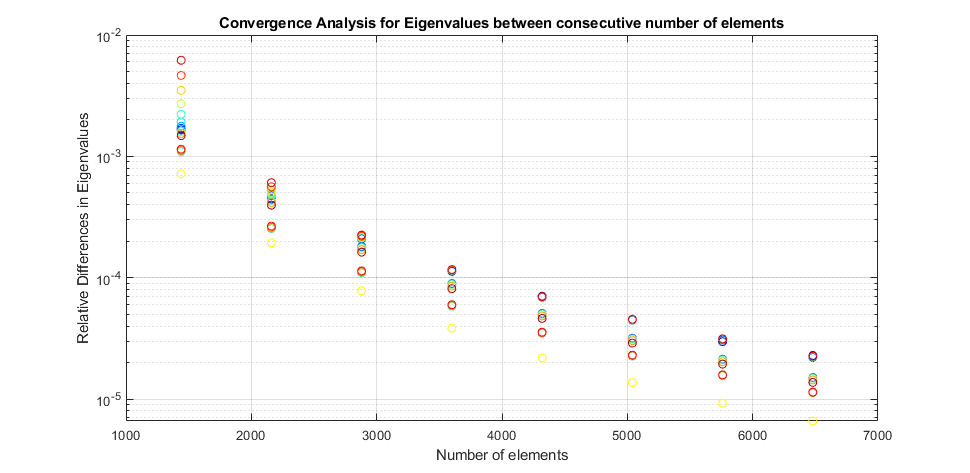
\includegraphics[scale=0.7]{convergence3d.png}
    \end{adjustbox}
    \caption{Rate of convergence of the first 20 eigenvalues.}
    \label{fig:conv_3d_eig}
\end{figure}

Similar to the two-dimensional case, the number of elements can be chosen so that at least the first 20 eigenvalues are accurate to 4 significant digits.

For the three-dimensional model, obtaining this level of accuracy can be difficult and computationally expensive. For the two-dimensional beam in Section \ref{sec:validity-of-a-cantilever-timoshenko-beam} and the upcoming two-dimensional plate model in Section \ref{sec:validity-of-a-plate} it is easier to get 5 significant digits of accuracy.

\subsection{Comparing the mode shapes}
To be able to compare the eigenvalues, the mode shapes of the two models are compared to match up the eigenvalues of the two models. This is the same approach as in Section \ref{sec:validity-of-a-cantilever-timoshenko-beam}. 

As seen in Section \ref{sec:validity-of-a-cantilever-timoshenko-beam}, the two-dimensional model as eigenvalues and eigenvectors that are not related to beam type problems. This is also true for the three-dimensional model, and it has even more non-beam type eigenvalues.

The focus of the investigation remains on beam type problems. Below are some examples of the mode shapes for beam type eigenvalues, mode shapes for non-beam type eigenvalues that are shared between the two and three-dimensional models and also mode shapes for non-beam type eigenvalues that are only present in the three-dimensional model.

\subsubsection{Mode shapes relating to beam type eigenvalues.}
Figure \ref{fig:beam-2dv3d} show some examples of beam type mode shapes for the displacement $u$.

\begin{figure}[h!]
	\scalebox{.8}{
		\makebox[\textwidth][c]{
			\centering
			\begin{minipage}[b]{0.8\linewidth}
				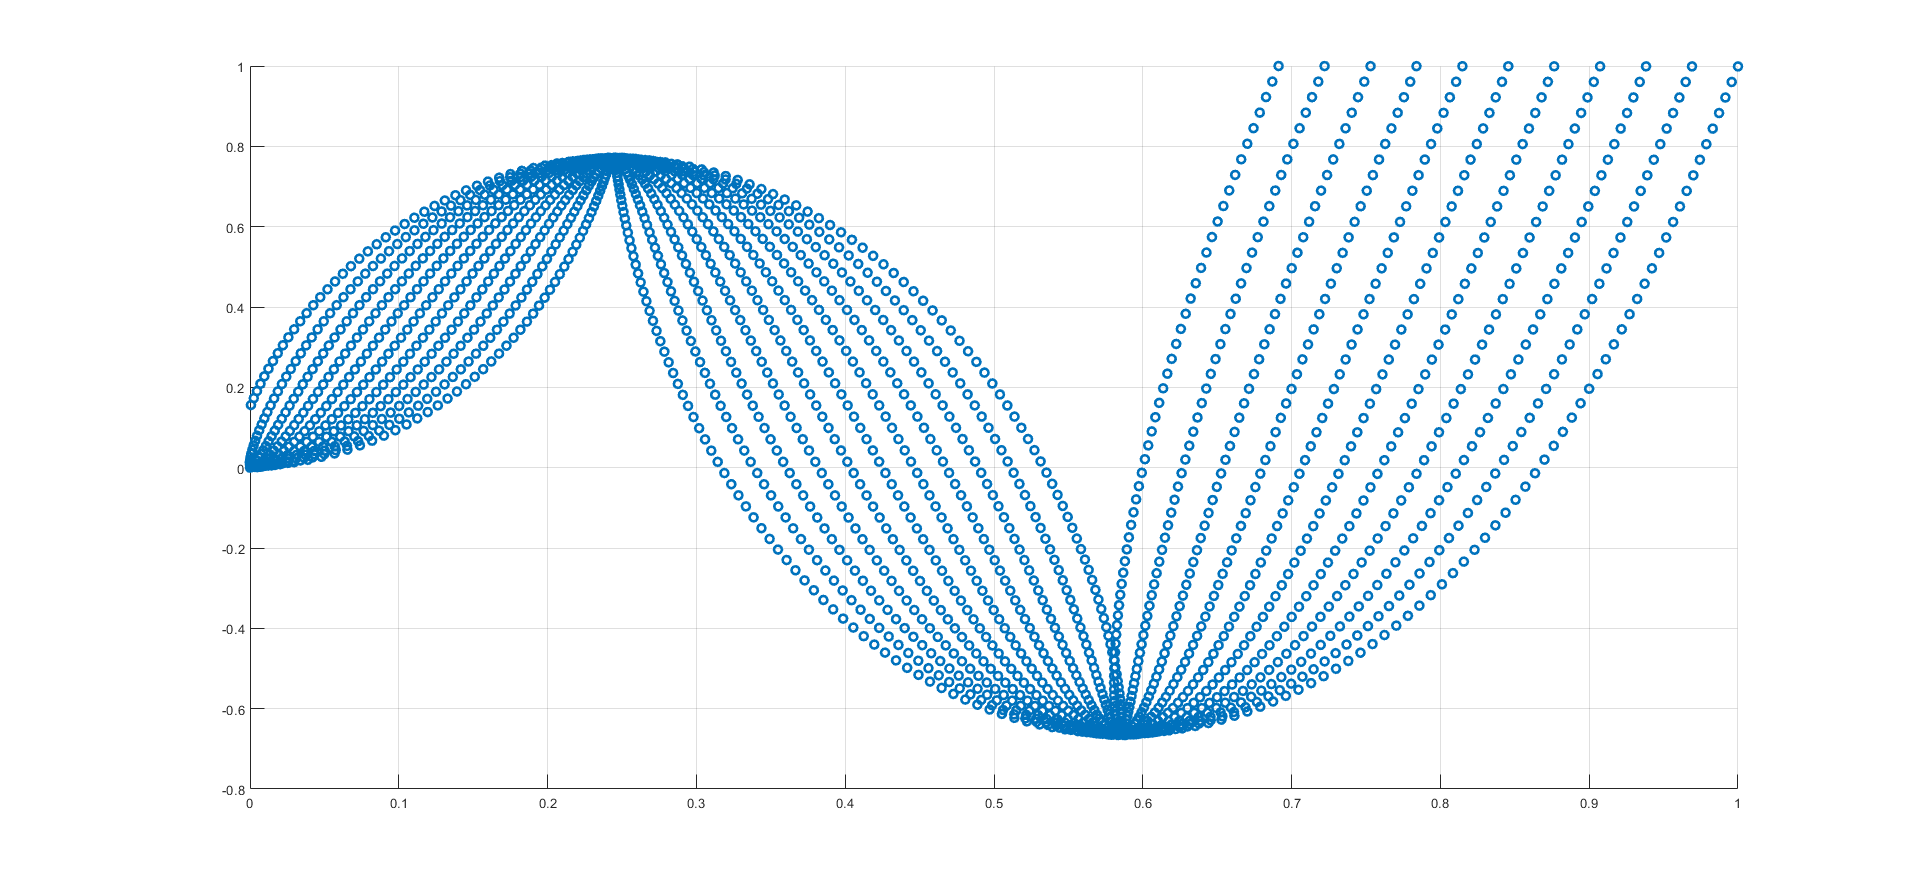
\includegraphics[width=1\linewidth]{3D12.png}
				\subcaption{3D Beam Type - $\lambda_{12} = 2.3293$}
				\label{fig:minipage2}
			\end{minipage}
			\begin{minipage}[b]{0.8\linewidth}
				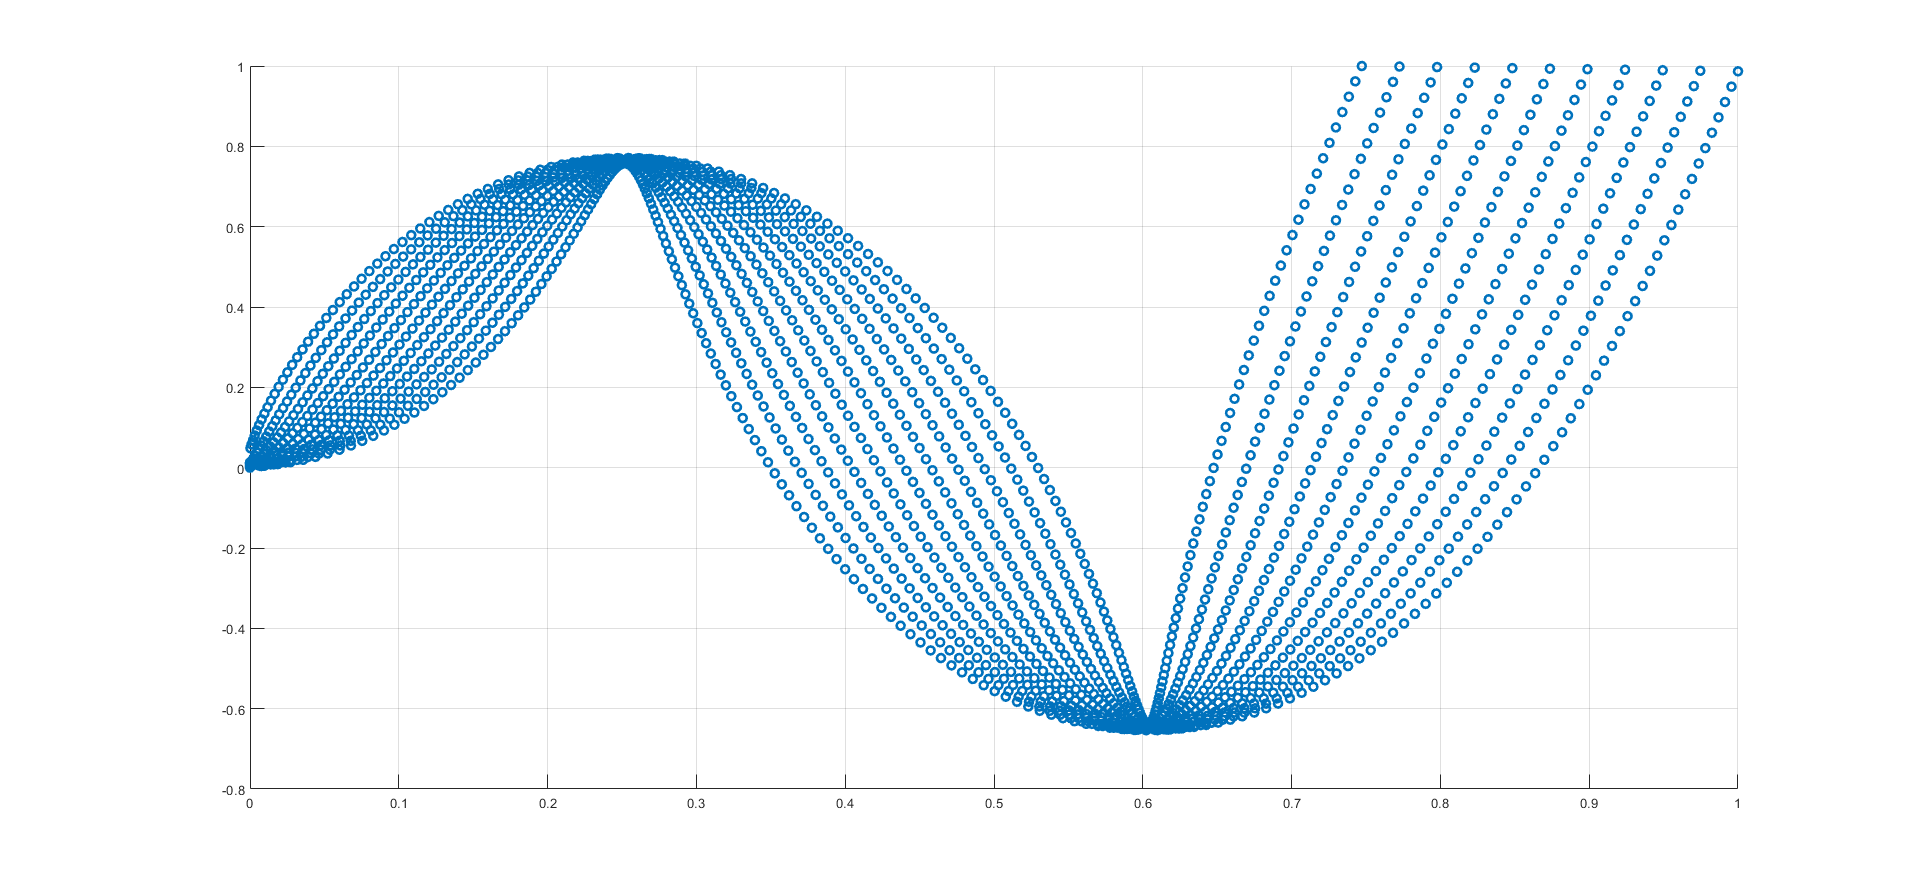
\includegraphics[width=1\linewidth]{2D3.png}
				\subcaption{2D Beam Type - $\lambda_3 = 2.3273$}
				\label{fig:minipage1}
			\end{minipage}
	}}
	\scalebox{.8}{
		\makebox[\textwidth][c]{
			\centering
			\begin{minipage}[b]{0.8\linewidth}
				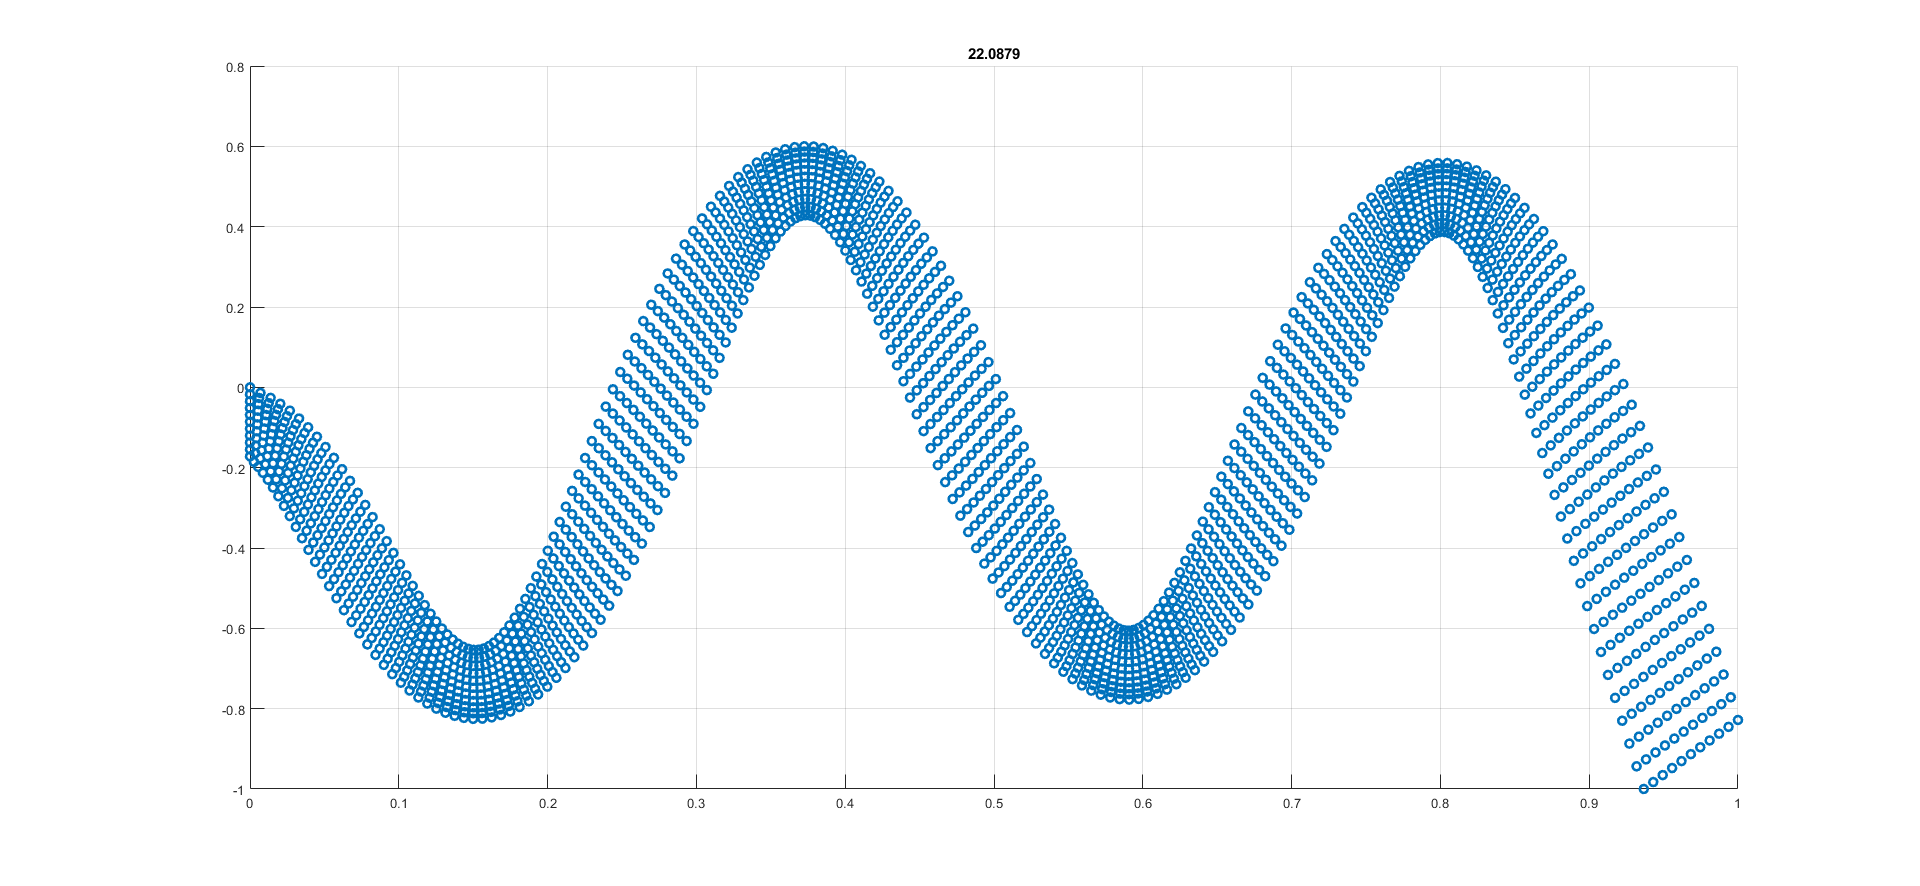
\includegraphics[width=1\linewidth]{3D22.png}
				\subcaption{3D Beam Type - $\lambda_{24} = 21.929$}
				\label{fig:minipage2}
			\end{minipage}
			\begin{minipage}[b]{0.8\linewidth}
				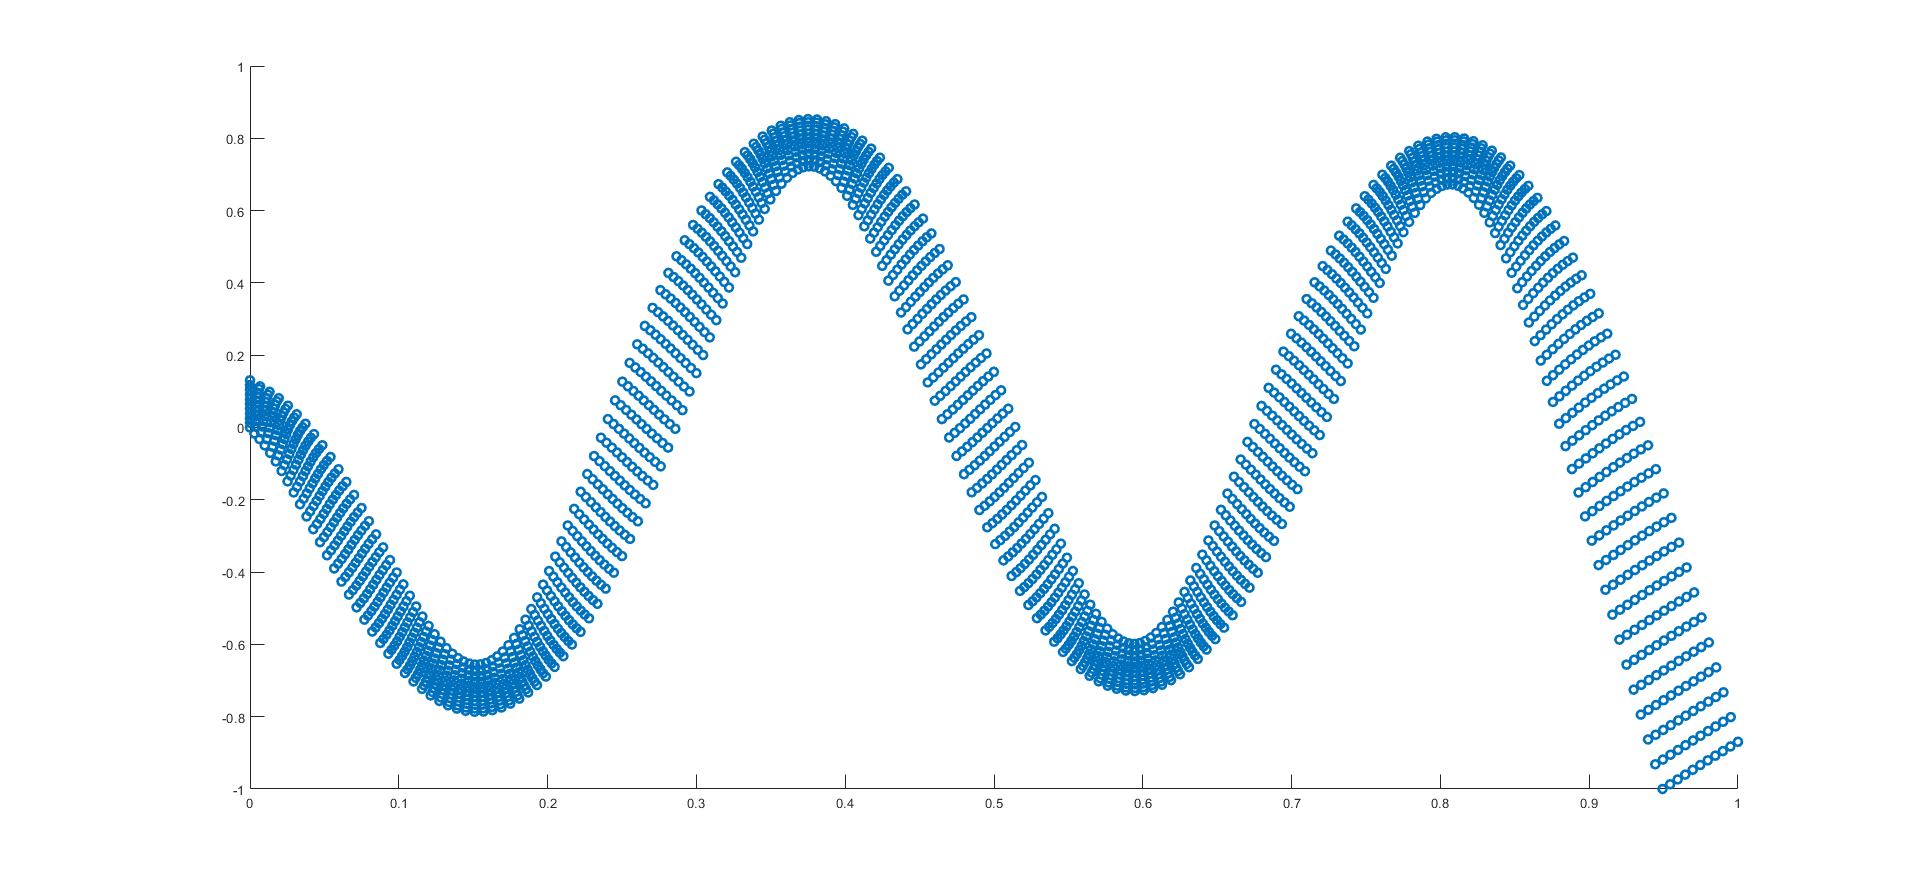
\includegraphics[width=1\linewidth]{2D6.png}
				\subcaption{2D Beam Type - $\lambda_6 = 21.911$}
				\label{fig:minipage1}
			\end{minipage}
			\caption{Mode shapes of the displacement $u$ with $h=1/20$.}
			\label{fig:beam-2dv3d}
	}}
\end{figure}
\FloatBarrier

\subsubsection{Mode shapes relating to non-beam type eigenvalues that are present in the two-dimensional model.}
Figure \ref{fig:nonbeam-2dv3d} show examples of mode shapes relating to non-beam type eigenvalues for the displacement $u$.

\FloatBarrier
\begin{figure}[h!]
	\scalebox{.8}{
		\makebox[\textwidth][c]{
			\centering
			\begin{minipage}[b]{0.8\linewidth}
				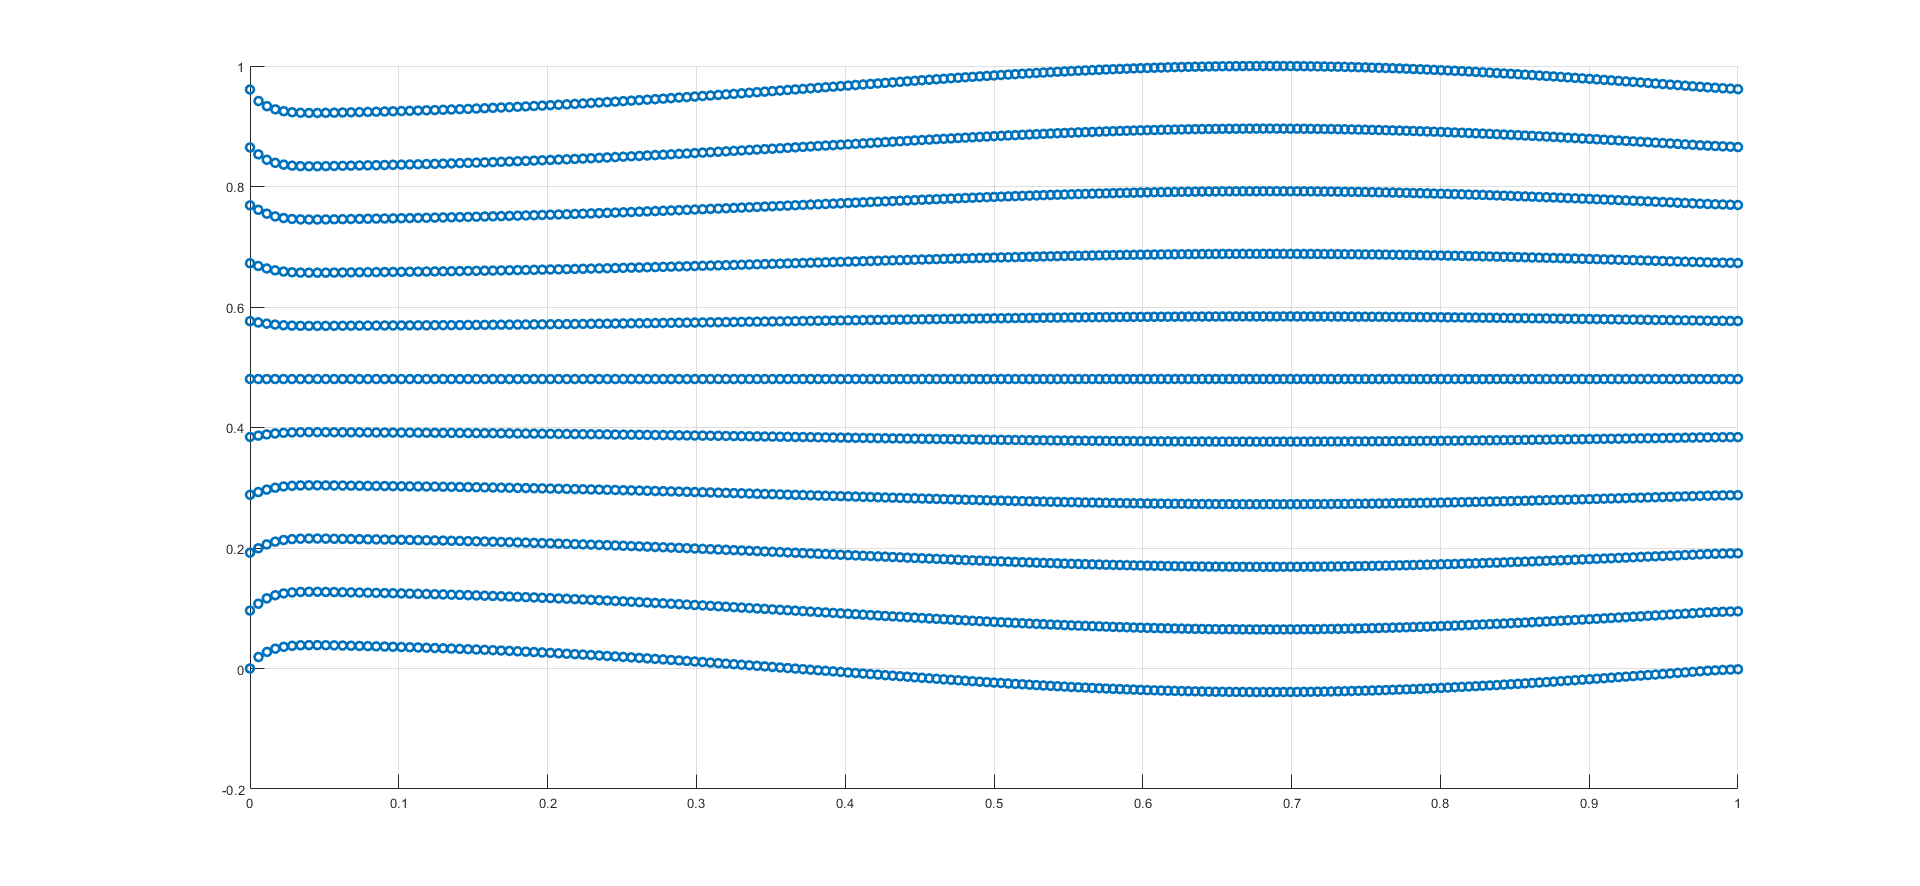
\includegraphics[width=1\linewidth]{3D33.png}
				\subcaption{3D Non-Beam Type - $\lambda_{33} = 69.374$}
				\label{fig:minipage2}
			\end{minipage}
			\begin{minipage}[b]{0.8\linewidth}
				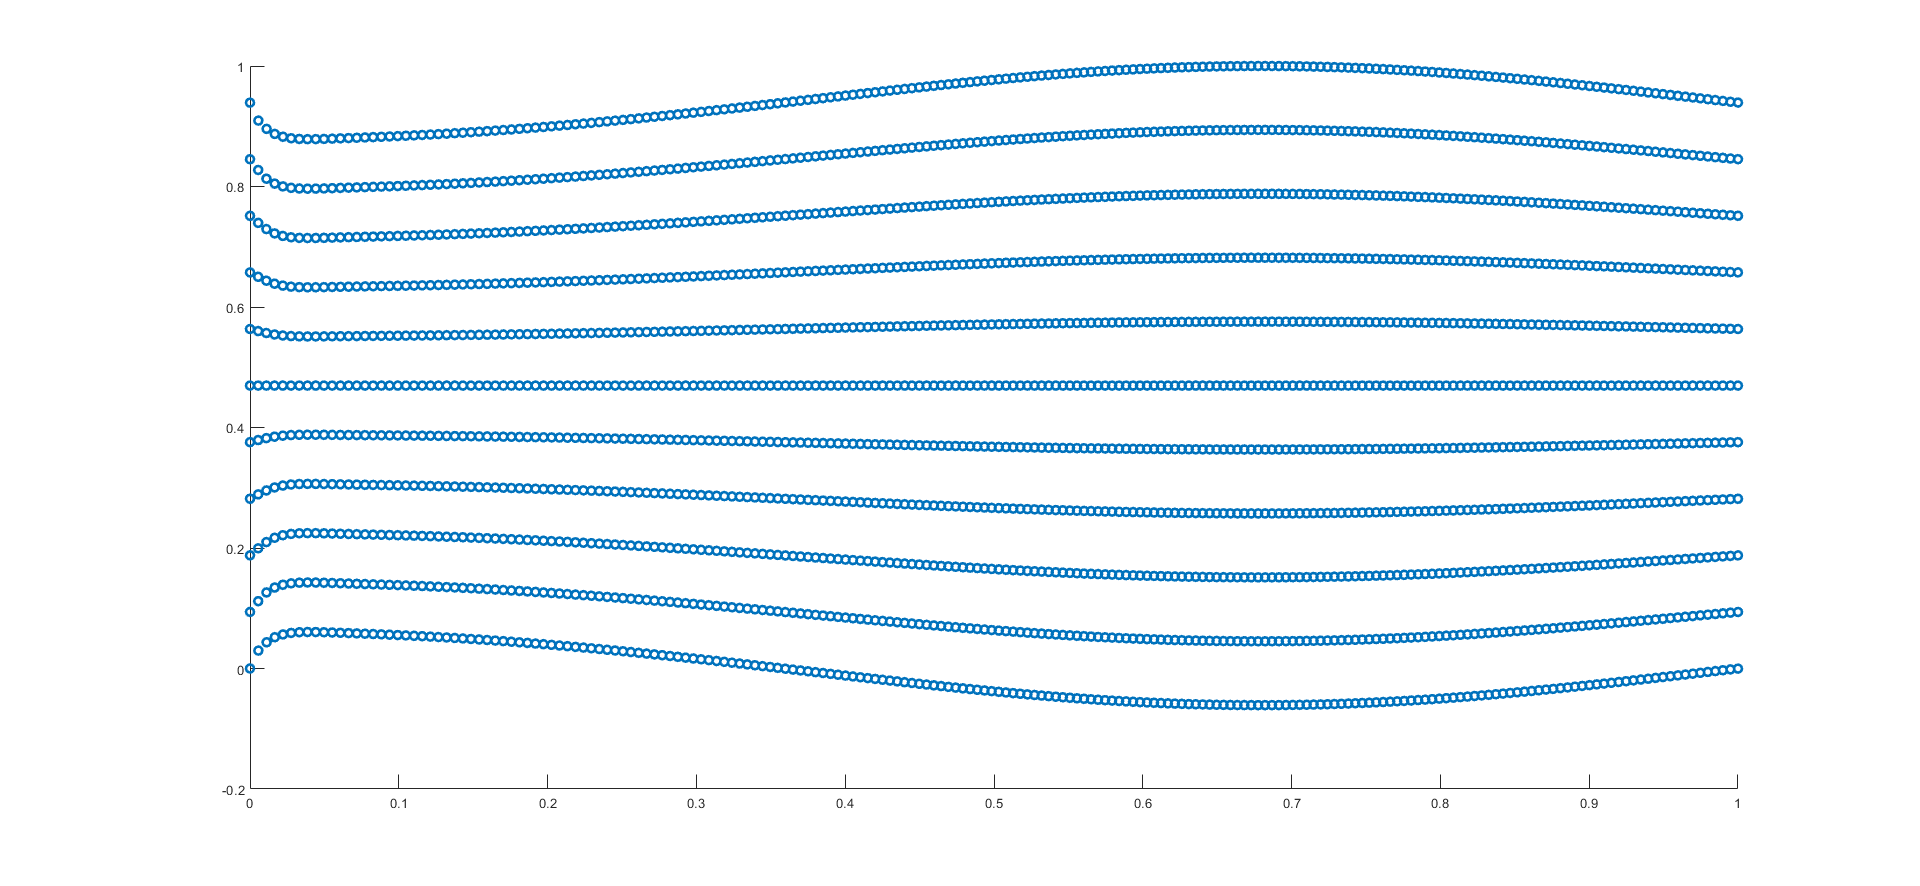
\includegraphics[width=1\linewidth]{2D8.png}
				\subcaption{2D Non-Beam Type - $\lambda_8 = 69.344$}
				\label{fig:minipage1}
			\end{minipage}
			\caption{Mode shapes of the displacement $u$ with $h=1/20$.}
			\label{fig:nonbeam-2dv3d}
	}}
\end{figure}
\FloatBarrier

\subsubsection{Mode shapes relating to non-beam type eigenvalues that are not present in the two-dimensional model.}
Figure \ref{fig:nonbeam-2dv3d} show examples of mode shapes relating to non-beam type eigenvalues for the displacement $u$ which are not present in the two-dimensional model. These mode shapes only appear in the three-dimensional beam.
\FloatBarrier
\begin{figure}[h!]
	\scalebox{.8}{
		\makebox[\textwidth][c]{
			\centering
			\begin{minipage}[b]{0.8\linewidth}
				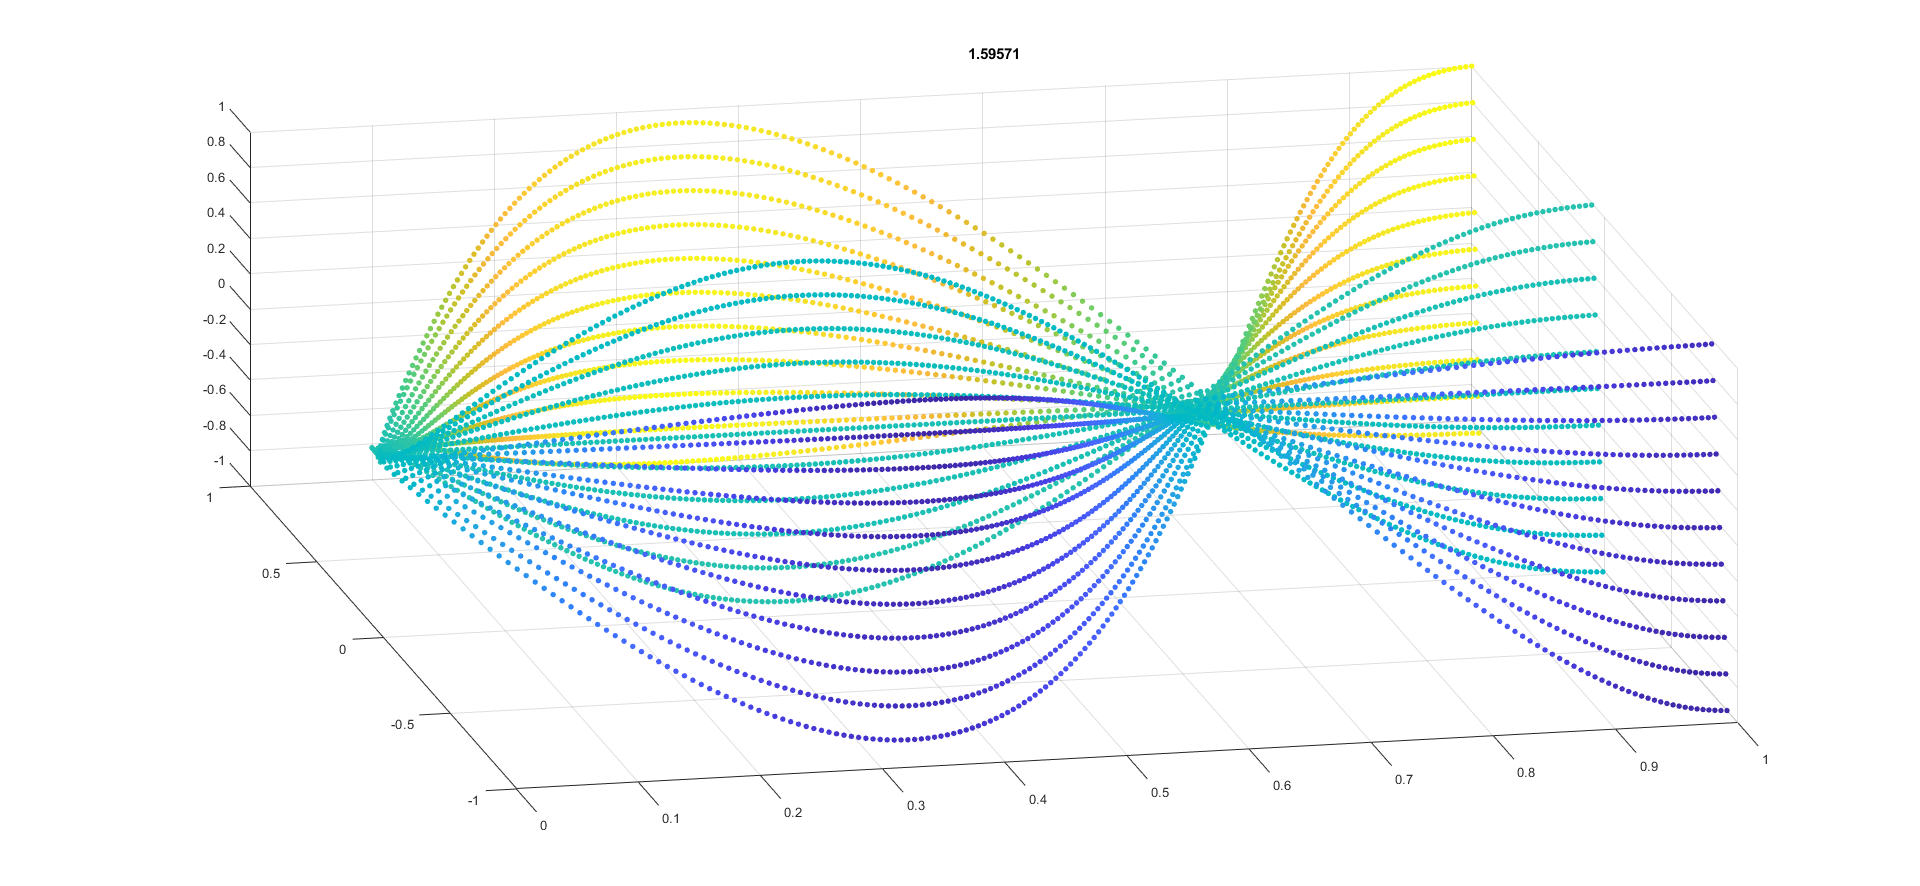
\includegraphics[width=1\linewidth]{3DNonBeam10.png}
				\subcaption{Non-2D Type - $\lambda_{10}$}
				\label{fig:minipage2}
			\end{minipage}
			\begin{minipage}[b]{0.8\linewidth}
				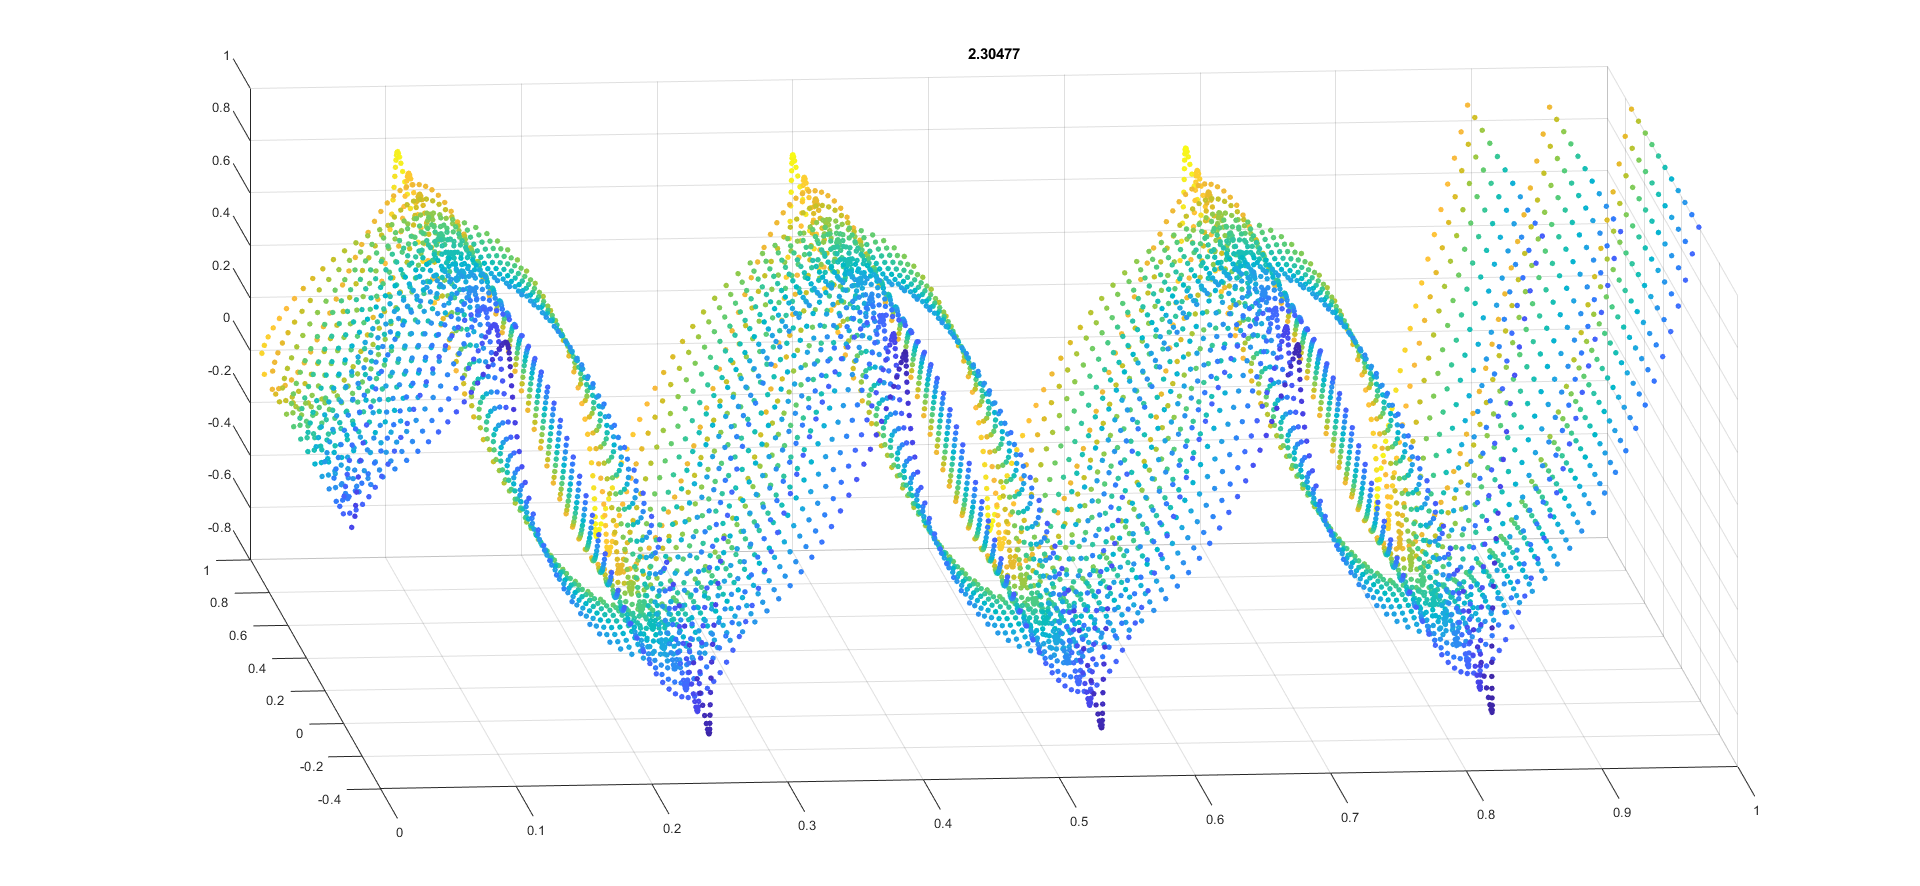
\includegraphics[width=1\linewidth]{3DNonBeam11.png}
				\subcaption{Non-2D Type - $\lambda_{11}$}
				\label{fig:minipage11}
			\end{minipage}
			\caption{Mode shapes of the displacement $u$ with $h=1/20$.}
			
	}}
\end{figure}
\FloatBarrier

\subsection{Comparing the eigenvalues}
For a realistic comparison of the models, the parameters need to be chosen carefully. The parameters are $h$ representing the height of the beam and $b$ representing the width of the beam. The two-dimensional model does not have the width parameter.

For $h$, the values used in Section \ref{sec:validity-of-a-cantilever-timoshenko-beam} will be used. These values covers a range of beam shapes from a short thick beam, to a long slender beam. two cases are selected that represents realistic cases. For a short and thick beam, consider $h = 1/5$ and for a long and slender beam, consider $h = 1/20$.

For the parameter $b$, two different cases will be considered. The first case is for $b \leq h$, and the $b > h$. The distinction of these two cases will become apparent in the results. It is important to note that the parameter $b$ will be expressed as a multiple of $h$.

All of the results will include all the eigenvalues shared between the two-models, including non-beam type eigenvalues. The non-beam type eigenvalues will be highlighted in grey. The non-beam type eigenvalues that are not shared between the two models will be excluded from the results, but the numbering of the eigenvalues will be kept as if they were included.

\subsubsection*{Case $b \leq h$:}
Table \ref{tab:2v3_1} below compares the eigenvalues of the models for a beam with a small length to height ratio of $h=1/5$ with decreasing values of $b$. 

\begin{table}[htbp]
	\scalebox{.8}{
	\makebox[\textwidth]{
		\caption{Comparsion of Eigenvalues with $h = 1/5$, with decreasing $b$ and $b < h$.}
		\begin{tabular}{|cc|cc|cc|cc||cc|}
			\hline
			\multicolumn{10}{|c|}{Eigenvalues} \\
			\hline
			\hline
			i     & {b = h} & i     & {b = 1/2 h} & i     & {b = 1/4 h} & i     & {b = 1/8 h} & j     & 2D \\
			\hline
			{2} & 0.12307 & {2} & 0.12234 & {2} & 0.12198 & {3} & 0.12178 & 1     & 0.12151 \\
			{3} & 3.5773 & {5} & 3.5630 & {6} & 3.5558 & {8} & 3.5519 & 2     & 3.5460 \\
			\rowcolor{lightgray}{5} & 7.7799 & {6} & 7.7596 & {8} & 7.7471 & {11} & 7.7401 & 3     & 7.7311 \\
			{8} & 20.334 & {9} & 20.283 & {11} & 20.26 & {14} & 20.247 & 4     & 20.225 \\
			{10} & 56.247 & {12} & 56.173 & {15} & 56.156 & {22} & 56.142 & 5     & 56.109 \\
			\rowcolor{lightgray}{11} & 69.197 & {14} & 69.319 & {17} & 69.281 & {24} & 69.238 & 6     & 69.164 \\
			{14} & 114.03 & {16} & 114.01 & {20} & 114.05 & {29} & 114.06 & 7     & 114.03 \\
			\rowcolor{lightgray}{17} & 187.01 & {19} & 189.14 & {25} & 189.37 & {36} & 189.34 & 8     & 189.17 \\
			{18} & 192.21 & {20} & 192.41 & {26} & 192.58 & {37} & 192.63 & 9     & 192.61 \\
			{21} & 284.76 & {23} & 285.43 & {31} & 285.74 & {42} & 285.84 & 10    & 285.85 \\
			{23} & 327.57 & {26} & 328.24 & {35} & 328.37 & {46} & 328.40 & 11    & 328.40 \\
			\rowcolor{lightgray}{25} & 347.77 & {28} & 356.44 & {36} & 357.30 & {50} & 357.33 & 12    & 357.08 \\
			{27} & 393.69 & {30} & 396.84 & {38} & 397.28 & {53} & 397.37 & 13    & 397.33 \\
			{30} & 434.46 & {34} & 441.05 & {41} & 441.81 & {57} & 441.99 & 14    & 442.00 \\
			\rowcolor{lightgray}{31} & 523.65 & {36} & 534.04 & {43} & 534.17 & {63} & 534.03 & 15    & 533.71 \\
			{34} & 550.51 & {37} & 537.82 & {44} & 538.86 & {64} & 539.06 & 16    & 538.97 \\
			\rowcolor{lightgray}{37} & 590.86 & {41} & 587.43 & {48} & 594.17 & {65} & 595.58 & 17    & 596.06 \\
			{39} & 590.86 & {42} & 600.52 & {49} & 602.25 & {67} & 602.69 & 18    & 602.77 \\
			\rowcolor{lightgray}{42} & 646.21 & {44} & 657.22 & {50} & 658.04 & {71} & 658.06 & 19    & 657.87 \\
			{44} & 711.07 & {46} & 714.62 & {53} & 717.10 & {73} & 717.51 & 20    & 717.37 \\
			\hline
			\hline
			\multicolumn{2}{|c|}{Max RE: \  2.6069\%} &\multicolumn{2}{c|}{Max RE: \ 1.4469\%}  & \multicolumn{2}{c|}{Max RE: \  0.38192\%}  & \multicolumn{2}{c||}{Max RE: \ 0.22301\%}& \multicolumn{2}{c|}{-} \\
			\hline
		\end{tabular}%
		\label{tab:2v3_1}%
	}}
\end{table}%
\FloatBarrier
\label{sym:RE}

% Table generated by Excel2LaTeX from sheet 'Sheet2'
\begin{table}[htbp]
	\centering
	\caption{Maximum relative error for beam type and non-beam type eigenvalues for $h = 1/5$.}
	\begin{tabular}{|c|cccc|}
		\hline
		\multicolumn{5}{|c|}{Maximum Relative Error} \\
		\hline
		\hline
		& {b = h} & {b = 1/2h} & {b = 1/4h} & {b = 1/8h} \\
		\hline
		Beam Type & 2.1420 \% & 0.6804 \% & 0.38192 \% & 0.22301 \% \\
		Non-Beam Type & 2.6069 \% & 1.4469 \% & 0.31546 \% & 0.11680 \% \\
		\hline
	\end{tabular}%
	\label{tab:2Dv3D_1_breakup}%
\end{table}%

Table \ref{tab:2v3_1} below compares the eigenvalues of the models for a beam with a larger length to height ratio of $h=1/20$ with decreasing values of $b$. 

\begin{table}[ht]
	\scalebox{.8}{
	\makebox[\textwidth]{
	\caption{Comparsion of Eigenvalues with $h = 1/20$, with decreasing $b$ and $b < h$.}
	\begin{tabular}{|cc|cc|cc|cc||cc|}
		\hline
		\multicolumn{10}{|c|}{Eigenvalues} \\
		\hline
		\hline
		i     & {b = h} & i     & {b = 1/2 h} & i     & {b = 1/4 h} & i     & {b = 1/8 h} & j     & 2D \\
		\hline
		{2} & 0.008043 & {2} & 0.008029 & {2} & 0.008023 & {3} & 0.00802 & {1} & {0.008013} \\
		{3} & 0.3087 & {4} & 0.30816 & {5} & 0.30794 & {7} & 0.30785 & {2} & {0.30757} \\
		{5} & 2.3357 & {8} & 2.3316 & {9} & 2.3300  & {12} & 2.3293 & {3} & {2.3273} \\
		\rowcolor{lightgray}{8} & 7.7217 & {10} & 7.7156 & {13} & 7.7124 & {16} & 7.7111 & {4} & {7.7077} \\
		{10} & 8.5387 & {11} & 8.5238 & {14} & 8.5182 & {18} & 8.516 & {5} & {8.5086} \\
		{11} & 21.986 & {14} & 21.948 & {18} & 21.934 & {24} & 21.929 & {6} & {21.911} \\
		{14} & 45.863 & {18} & 45.781 & {21} & 45.756 & {30} & 45.746 & {7} & {45.712} \\
		\rowcolor{lightgray}{17} & 69.444 & {19} & 69.408 & {25} & 69.385 & {33} & 69.374 & {8} & {69.344} \\
		{18} & 83.149 & {22} & 82.999 & {27} & 82.960 & {36} & 82.944 & {9} & {82.887} \\
		{21} & 136.44 & {25} & 136.19 & {31} & 136.14 & {42} & 136.12 & {10} & {136.03} \\
		\rowcolor{lightgray}{23} & 192.62 & {27} & 192.62 & {35} & 192.58 & {47} & 192.56 & {11} & {192.48} \\
		{25} & 207.87 & {29} & 207.5 & {36} & 207.43 & {48} & 207.41 & {12} & {207.29} \\
		{27} & 299.14 & {33} & 298.63 & {41} & 298.56 & {55} & 298.53 & {13} & {298.38} \\
		\rowcolor{lightgray}{30} & 376.68 & {35} & 377.01 & {44} & 377.01 & {58} & 376.98 & {14} & {376.83} \\
		{31} & 411.58 & {37} & 410.89 & {46} & 410.83 & {61} & 410.81 & {15} & {410.63} \\
		{34} & 546.15 & {40} & 545.27 & {50} & 545.24 & {66} & 545.23 & {16} & {545.03} \\
		\rowcolor{lightgray}{37} & 620.77 & {42} & 622.02 & {53} & 622.19 & {69} & 622.18 & {17} & {621.95} \\
		{39} & 703.55 & {44} & 702.49 & {54} & 702.29 & {71} & 702.53 & {18} & {702.31} \\
		{42} & 884.27 & {47} & 883.02 & {59} & 883.14 & {82} & 883.19 & {19} & {882.96} \\
		\rowcolor{lightgray}{44} & 923.68 & {49} & 926.88 & {60} & 927.43 & {86} & 927.50 & {20} & {927.18} \\
		\hline
		\hline
		\multicolumn{2}{|c|}{Max RE: \  0.37701\%} &\multicolumn{2}{c|}{Max RE: \ 0.19893\%}  & \multicolumn{2}{c|}{Max RE: \  0.12393\%}  & \multicolumn{2}{c||}{Max RE: \ 0.092843\%}& \multicolumn{2}{c|}{-} \\
		\hline
	\end{tabular}%
	\label{tab:2v3_2}%
}}
\end{table}%
\FloatBarrier

\begin{table}[htbp]
	\centering
	\caption{Maximum relative error for beam type and non-beam type eigenvalues for $h = 1/20$}
	\begin{tabular}{|c|cccc|}
		\hline
		\multicolumn{5}{|c|}{Maximum Relative Error} \\
		\hline
		\hline
		& {b = h} & {b = 1/2h} & {b = 1/4h} & {b = 1/8h} \\
		\hline
		Beam Type & 0.37701 \% & 0.19893 \% & 0.12393 \% & 0.092843 \% \\
		Non-Beam Type & 0.37682 \% & 0.10218 \% & 0.061213 \% & 0.043601 \% \\
		\hline
	\end{tabular}%
	\label{tab:2v3_2_split}%
\end{table}%
\FloatBarrier

Tables \ref{tab:2v3_1} and \ref{tab:2v3_2} show that the first 20 eigenvalues of the two-dimensional model compares very well to the matching eigenvalues of the three-dimensional beam for $b \leq h$. As the width $b$ decreases, the two-dimensional model becomes a better approximation of the three-dimensional model. Also shown is that the slender beam with $h = 1/20$ compares better than the thick beam where $h = 1/5$, event though the case of $h=1/5$ is still a very good comparison. 

The tables also shows that the three-dimensional model has more non-beam type eigenvalues as the width $b$ decreases, as well as when the width $h$ decreases.This is different from the two-dimensional model as seen in \ref{sec:validity-of-a-cantilever-timoshenko-beam}.

Tables \ref{tab:2Dv3D_1_breakup} and \ref{tab:2v3_2_split} breaks up the maximum relative error for the beam type and non-beam type eigenvalues. These tables confirm that the the beam type eigenvalues compare very well.


\subsubsection*{Case $b > h$:}
First, the case is considered where $h = 1/5$.

\FloatBarrier
\begin{table}[htbp]
	\scalebox{.8}{
	\makebox[\textwidth]{
		\caption{Comparsion of Eigenvalues with $h = 1/5$, with increasing $b$ and $b > h$}
		\begin{tabular}{|cc|cc|cc||cc|}
			\hline
			\multicolumn{8}{|c|}{Eigenvalues} \\
			\hline
			\hline
			i     & {b = 2h} & i     & {b = 4h} & i     & {b = 8h} & j     & 2D \\
			\hline
			{1} & 0.12474 					& {1} & 0.12766 & {1} & 0.13036 & 1     & 0.12151 \\
			{4} & 3.6088 					& {4} & 3.6297 & {5} & 3.7766 & 2     & 3.5460 \\
			\rowcolor{lightgray}{6} & 7.8091 & {5} & 7.8389 & {9} & 8.9239 & 3     & 7.7311 \\
			{8} & 20.466 					& {9} & 20.959 & {15} & 21.031 & 4     & 20.255 \\
			{11} & 56.309					& {18} & 58.149 & {30} & 60.862 & 5     & 56.109 \\
			\hline
			\hline
			\multicolumn{2}{|c|}{Max RE: \  2.6603\%} &\multicolumn{2}{c|}{Max RE: \ 5.0571\%}  & \multicolumn{2}{c|}{Max RE: \  15.428\%} & \multicolumn{2}{c|}{-} \\
			\hline
		\end{tabular}%
		\label{tab:b>h}%
	}}
\end{table}
\FloatBarrier

\FloatBarrier
\begin{table}[htbp]
	\centering
	\caption{Maximum relative error for beam type and non-beam type eigenvalues for $h = 1/5$}
	\begin{tabular}{|c|ccc|}
		\hline
		\multicolumn{4}{|c|}{Maximum Relative Error} \\
		\hline
		\hline
		& {b = 2h} & {b = 4h} & {b = 8h} \\
		\hline
		Beam Type & 2.6603 \% & 5.0571 \% & 8.4712 \% \\
		Non-Beam Type & 1.0096 \% & 1.3948 \% & 15.428 \% \\
		\hline
	\end{tabular}%
	\label{tab:b>h-split}%
\end{table}%
\FloatBarrier

In Table \ref{tab:b>h}, the height of the beam is set to $h=1/20$, which was the best case when $b<h$.

\FloatBarrier
\begin{table}[htbp]
	\scalebox{.8}{
	\makebox[\textwidth]{
		\caption{Comparsion of Eigenvalues with $h = 1/20$, with increasing $b$ and $b > h$}
		\begin{tabular}{|cc|cc|cc||cc|}
			\hline
			\multicolumn{8}{|c|}{Eigenvalues} \\
			\hline
			\hline
			i     & {b = 2h} & i     & {b = 4h} & i     & {b = 8h} & j     & 2D \\
			\hline
			{2} & 0.008076 & {1} & 0.008162 & {1} & 0.008324 & 1     & 0.008013 \\
			{3} & 0.30995 & {3} & 0.31298 & {3} & 0.31738 & 2     & 0.30757 \\
			{5} & 2.3462 & {5} & 2.3737 & {6} & 2.4116 & 3     & 2.3273 \\
			\rowcolor{lightgray}{8} & 7.7312 & {8} & 7.7471 & {9} & 7.7711 & 4     & 7.7077 \\
			{10} & 8.5841 & {9} & 8.7082 & {10} & 8.7929 & 5     & 8.5086 \\
			{11} & 22.124 & {12} & 22.491 & {14} & 23.222 & 6     & 21.911 \\
			{14} & 46.195 & {14} & 47.003 & {18} & 47.921 & 7     & 45.712 \\
			\rowcolor{lightgray}{17} & 69.454 & {17} & 69.281 & {22} & 72.307 & 8     & 69.344 \\
			{18} & 83.822 & {18} & 85.218 & {24} & 80.607 & 9     & 82.887 \\
			{21} & 137.43 & {21} & 138.58 & {32} & 140.97 & 10    & 136.03 \\
			\hline
			\hline
			\multicolumn{2}{|c|}{Max RE: \  1.1289\%} &\multicolumn{2}{c|}{Max RE: \ 2.8261\%}  & \multicolumn{2}{c|}{Max RE: \  5.9821\%} & \multicolumn{2}{c|}{-} \\
			\hline
		\end{tabular}%
		\label{tab:b>h_20}%
	}}
\end{table}
\FloatBarrier

\FloatBarrier
\begin{table}[htbp]
	\centering
	\caption{Maximum relative error for beam type and non-beam type eigenvalues for $h = 1/20$}
	\begin{tabular}{|c|ccc|}
		\hline
		\multicolumn{4}{|c|}{Maximum Relative Error} \\
		\hline
		\hline
		& {b = 2h} & {b = 4h} & {b = 8h} \\
		\hline
		Beam Type & 1.1289 \% & 2.8261 \% & 5.9821 \% \\
		Non-Beam Type & 0.30521 \% & 0.51096 \% & 4.2734 \% \\
		\hline
	\end{tabular}%
	\label{tab:b>h-split_20}%
\end{table}%
\FloatBarrier

Tables \ref{tab:b>h} and \ref{tab:b>h_20} show that the two-dimensional model compares not as well to the three-dimensional model when $b$ is larger than $h$. Tables \ref{tab:b>h-split} and \ref{tab:b>h-split_20} show that this is also true for the beam type eigenvalues.

For the case of $h=1/5$, it was also more difficult to obtain reliable eigenvalues using a numerical method.

These results give a detailed overview of the validity of the cantilever two-dimensional beam compared to the cantilever three-dimensional beam. The results show that the two-dimensional beam model compares very well to the three-dimensional beam model for a large range of beam shapes. The results shown were chosen to represent realistic cases, and the results are similar for other cases.

The overall conclusion is that the shape of the beam is very important. If the width $b$ is equal to or less than the height $h$, the two-dimensional beam model compares very well to the three-dimensional beam model. More so when the beam is slender, and less so when the beam is short and thick.

When the width $b$ is larger than the height $h$, the two-dimensional beam the comparison degrades very quickly. This is true for both slender and short and thick beams, although with short and thick beams, it is more difficult to obtain reliable eigenvalues using a numerical method.

For practical applications, if $b > h$ the use of a beam model must be brought into question. Other models such as a plate model will be better suited as it is a more realistic model. In the next section, the validity of the Reissner-Mindlin plate mode is investigated using the same method of this section.

\end{document}